\documentclass[11pt,a4wide]{article}
\usepackage{verbatim}
\usepackage{listings}
\usepackage{graphicx}
\usepackage{a4wide}
\usepackage{color}
\usepackage{amsmath}
\usepackage{amssymb}
\usepackage[dvips]{epsfig}
\usepackage[T1]{fontenc}
\usepackage{cite} % [2,3,4] --> [2--4]
\usepackage{shadow}
\usepackage{hyperref}

\setcounter{tocdepth}{2}

\lstset{language=c++}
\lstset{alsolanguage=[90]Fortran}
\lstset{basicstyle=\small}
\lstset{backgroundcolor=\color{white}}
\lstset{frame=single}
\lstset{stringstyle=\ttfamily}
\lstset{keywordstyle=\color{red}\bfseries}
\lstset{commentstyle=\itshape\color{blue}}
\lstset{showspaces=false}
\lstset{showstringspaces=false}
\lstset{showtabs=false}
\lstset{breaklines}
\begin{document}
\section*{Introduction to numerical projects}

Here follows a brief recipe and recommendation on how to write a report for each
project.
\begin{itemize}
\item Give a short description of the nature of the problem and the eventual 
numerical methods you have used.
\item Describe the algorithm you have used and/or developed. Here you may find it convenient
to use pseudocoding. In many cases you can describe the algorithm
in the program itself.

\item Include the source code of your program. Comment your program properly.
\item If possible, try to find analytic solutions, or known limits
in order to test your program when developing the code.
\item Include your results either in figure form or in a table. Remember to
       label your results. All tables and figures should have relevant captions
       and labels on the axes.
\item Try to evaluate the reliabilty and numerical stability/precision
of your results. If possible, include a qualitative and/or quantitative
discussion of the numerical stability, eventual loss of precision etc. 

\item Try to give an interpretation of you results in your answers to 
the problems.
\item Critique: if possible include your comments and reflections about the 
exercise, whether you felt you learnt something, ideas for improvements and 
other thoughts you've made when solving the exercise.
We wish to keep this course at the interactive level and your comments can help
us improve it.
\item Try to establish a practice where you log your work at the 
computerlab. You may find such a logbook very handy at later stages
in your work, especially when you don't properly remember 
what a previous test version 
of your program did. Here you could also record 
the time spent on solving the exercise, various algorithms you may have tested
or other topics which you feel worthy of mentioning.
\end{itemize}



\section*{Format for electronic delivery of report and programs}
%
This project counts 1/3 of the final mark. The feedback will, in addition to our comments contain a final score, where 100 is the maximum. Project 4 counts also 1/3 of the final mark. The final exam stands for the remaining 1/3 of the final mark.
We have set up devilry so that you can use your candidate number only. Please mark your project with the candidate number. If you prefer to not use the candidate number, we will need it anyway in order to correlate with the final written exam. 

The preferred format for the report is a PDF file. You can also
use DOC or postscript formats or as an ipython notebook file. 
As programming language we prefer that you choose between C/C++, Fortran2008 or Python.
The following prescription should be followed when preparing the report:
\begin{itemize}
\item Use Devilry to hand in your projects, log in  at 
\url{ http://devilry.ifi.uio.no} with your normal UiO username and password
and choose either 'fys3150' or 'fys4150'. This time however you should use your candidate number only. You are free to use your name as well, but we need the candidate number for the final mark. 
\item You can upload the report file as well as your program files to devilry!  For the source code file(s) you have developed you can also place these at  a github domain, or eventually upload all program files to devilry.  
The report file should include all of your discussions and a list of the codes you have developed. 
\item You should include tests and/or unit tests of your code(s).
\item Comments  from us on your projects, with final score
will be available under
your Devilry domain and are only visible to you and the teachers of the course.

\end{itemize}

Finally, even though this project counts 1/3 of the final mark, 
we encourage you to work two and two together. Optimal working groups consist of 
2-3 students. You can then hand in a common report. 


\section*{Project 5,Diffusion of neurotransmitters in the synaptic cleft,  deadline  Friday December 11}

The dominant way of transporting signals between neurons (nerve cells)
in the brain is by means of diffusion of particular signal molecules
called \emph{neurotransmitters} across the synaptic cleft separating
the cell membranes of the two cells. A drawing of a synapse is
given in Fig.~\ref{fig:figure1}.
\begin{figure}[thb]
\centerline{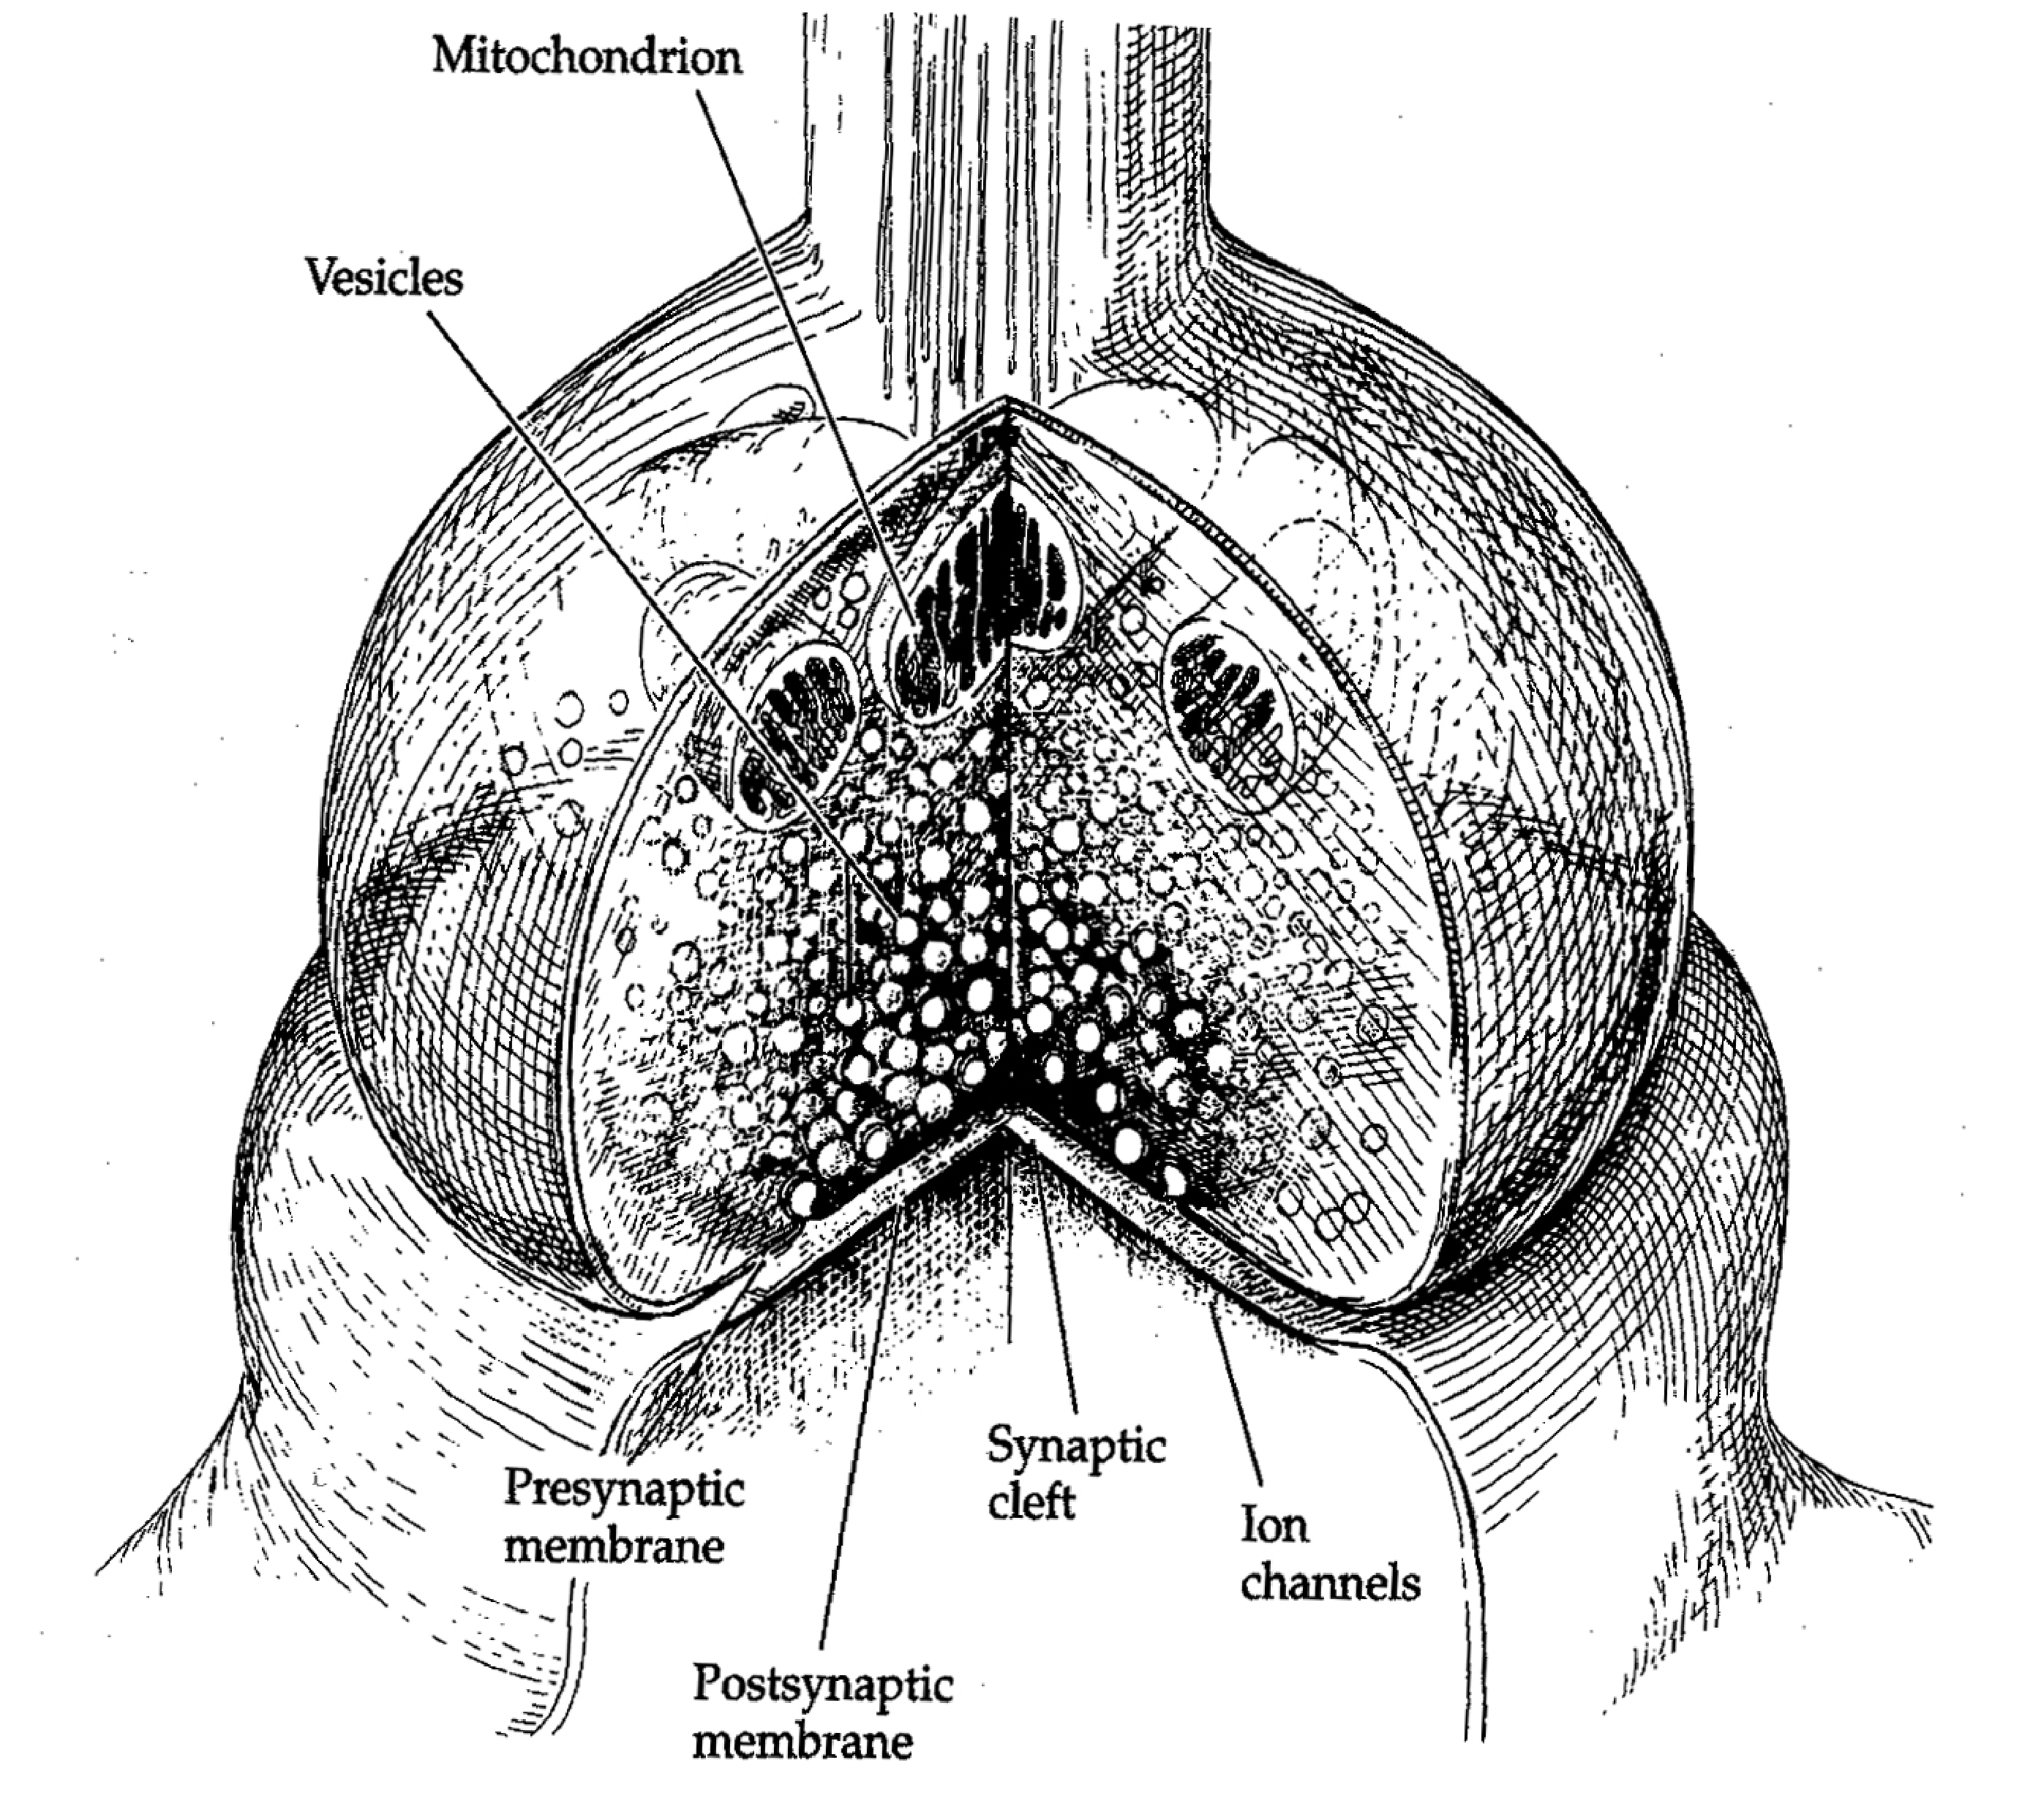
\includegraphics[width=9cm]{FigDiffusion/thompsonB2000-p38.eps}}
\caption{\small Drawing of a synapse. The axon terminal is the knoblike
structure and the spine of the receiving neuron is the bottom one. The
synaptic cleft is the small space between the presynaptic (axon)
and postsynaptic (dendritic spine) membrane.
(From Thompson: ``The Brain'', Worth Publ., 2000)}
\label{fig:figure1}
\end{figure}

Following the arrival of an action potential in the axon terminal a
process is initiated in which (i) vesicles inside the axon terminal
(filled with neurotransmitter molecules) merge with the presynaptic
(axon) membrane and (ii) release neurotransmitters into the synaptic
cleft. These neurotransmitters diffuse across the synaptic cleft to
receptors on the postsynaptic side which ``receives'' the signal.
A schematic illustration of this process is shown in
Fig.~\ref{fig:figure2}(left).
\begin{figure}[t]
\centerline{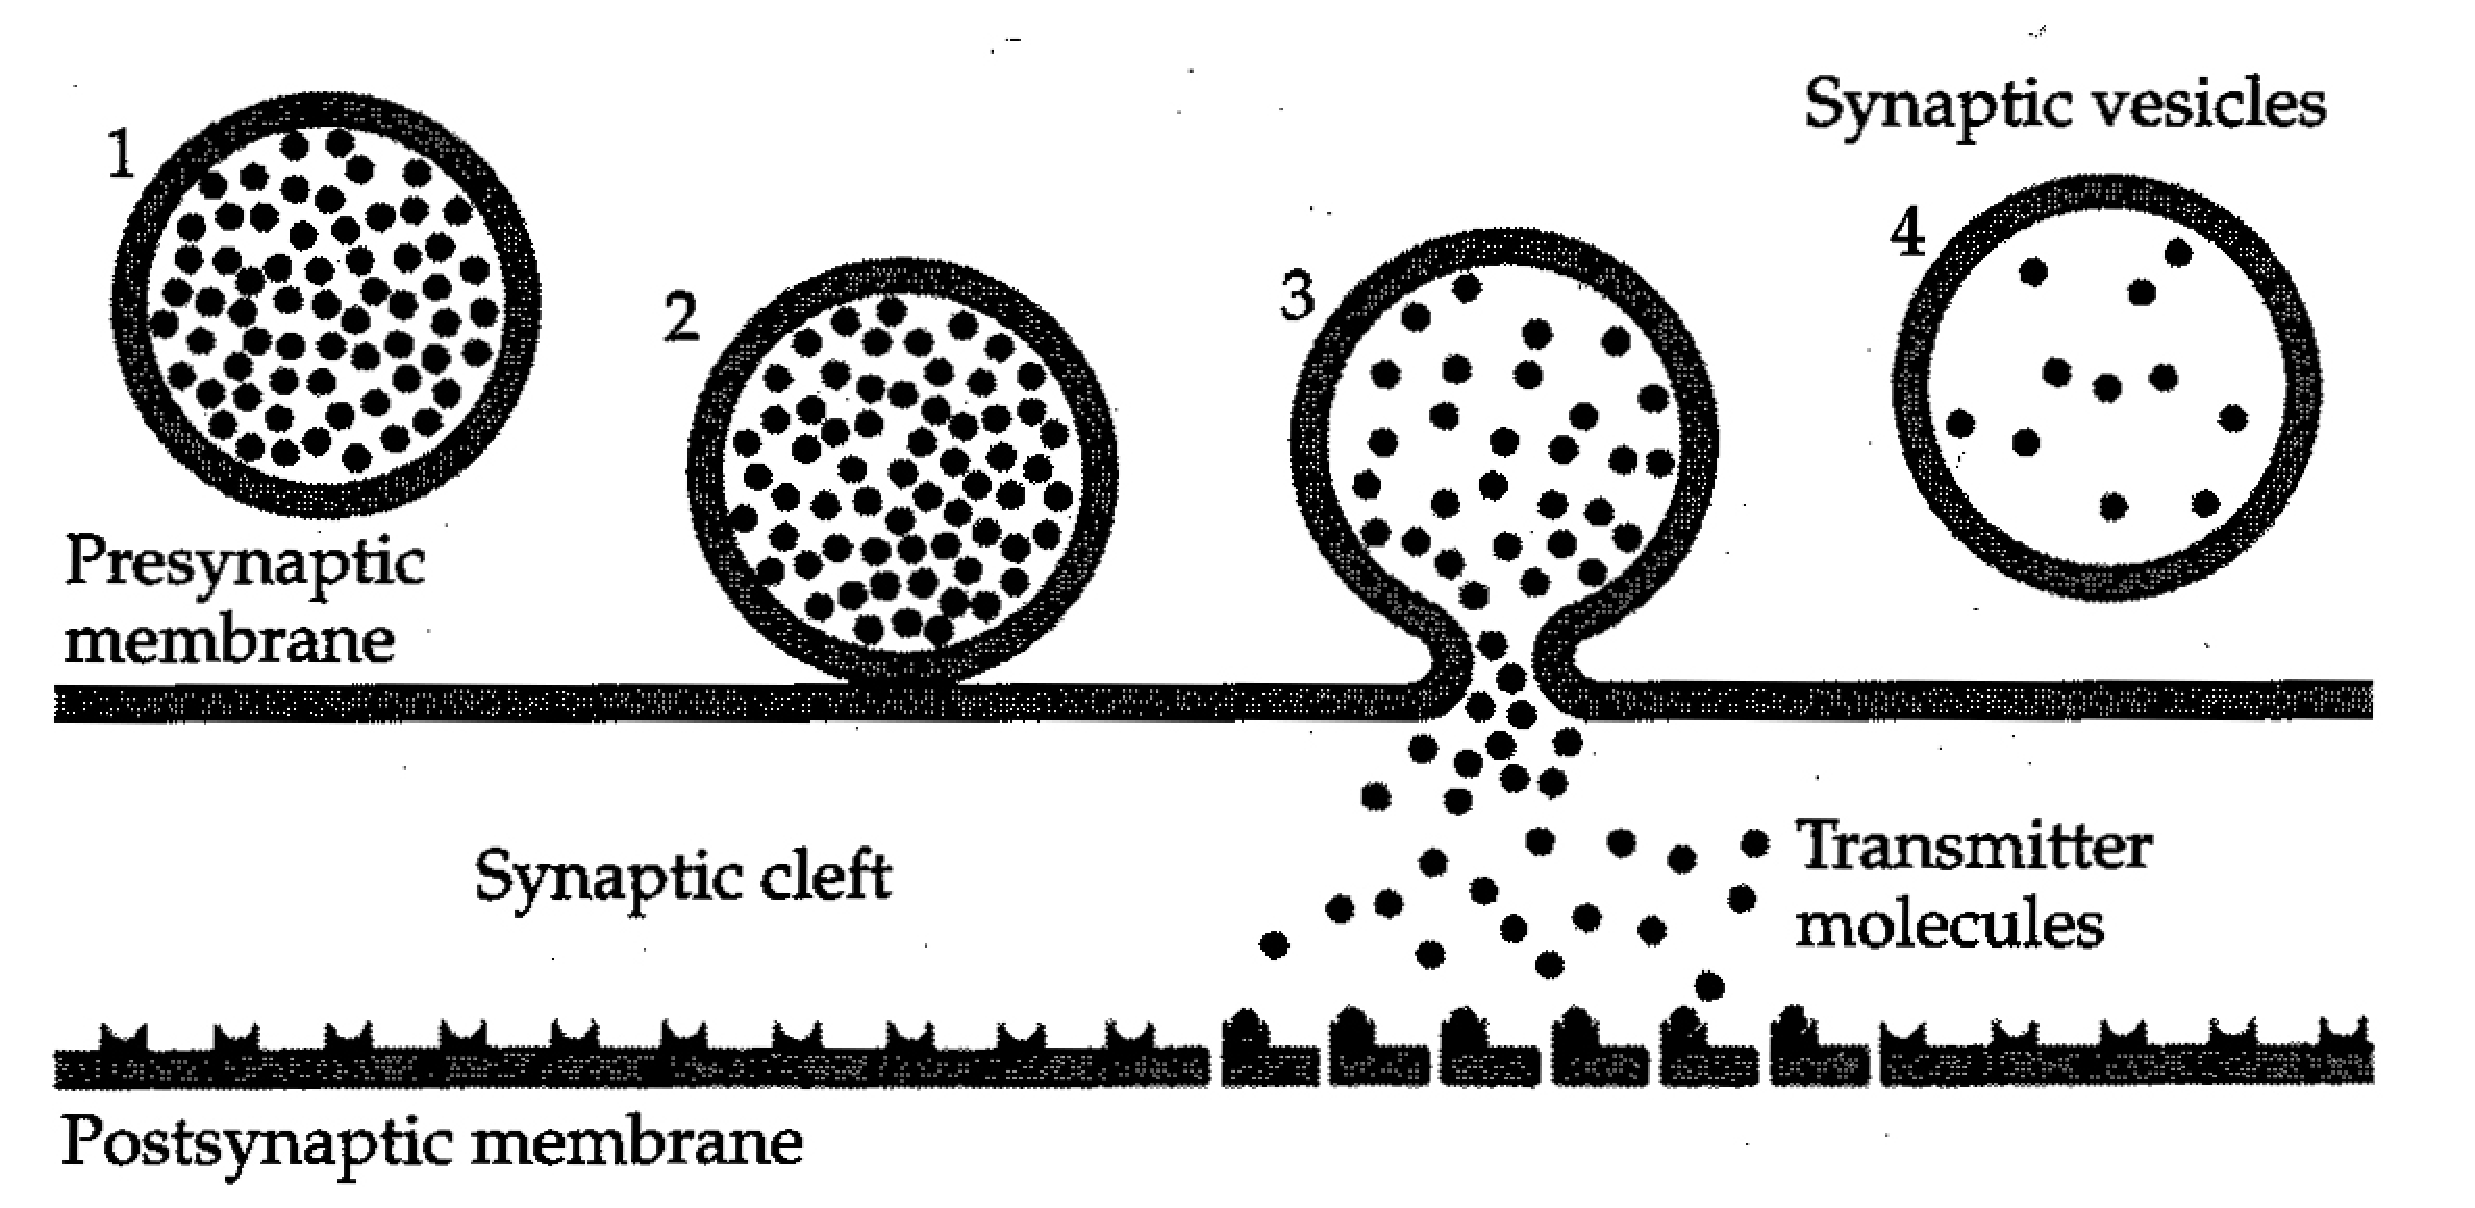
\includegraphics[width=10cm]{FigDiffusion/thompsonB2000-p39.eps}
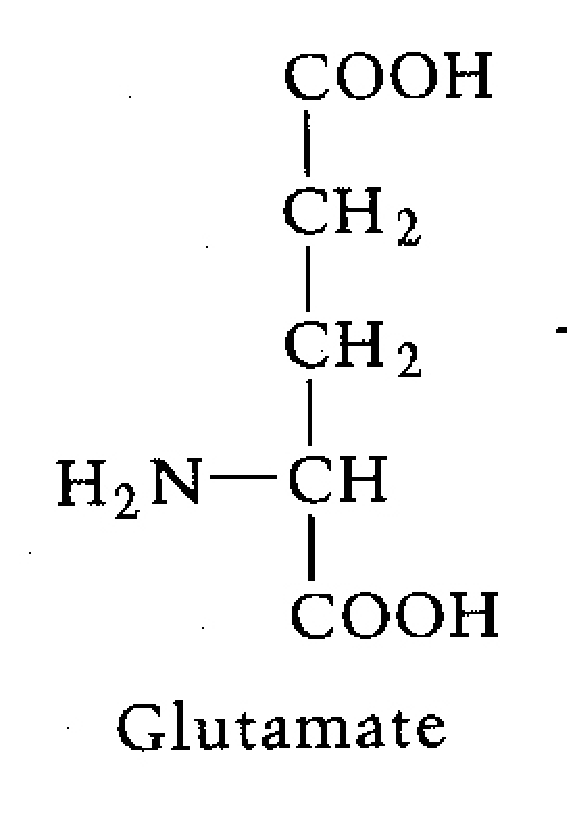
\includegraphics[width=3cm]{FigDiffusion/kandel-B1991-p217-glutamate.eps}
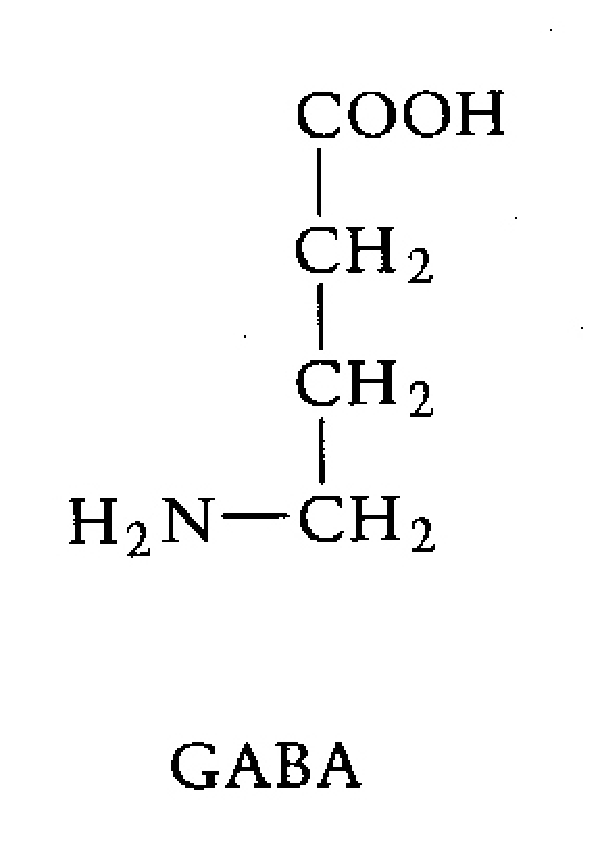
\includegraphics[width=3cm]{FigDiffusion/kandel-B1991-p217-GABA.eps}}
\caption{\small Left: Schematic drawing
of the process of vesicle release from the axon terminal and release of
transmitter molecules into the synaptic cleft. (From Thompson: ``The
Brain'', Worth Publ., 2000). Right: Molecular structure of the
two important neurotransmitters \emph{glutamate} and \emph{GABA}.}
\label{fig:figure2}
\end{figure}
Since the transport process in the synaptic cleft is governed by
diffusion, we can describe it mathematically by
%
\begin{equation}
\frac{\partial u}{\partial t} = D \nabla^2 u,
\label{eq:diffusion_eq_3D}
\end{equation}
%
where $u$ is the concentration of the particular neurotransmitter, and
$D$ is the diffusion coefficient of the neurotransmitter in this
particular environment (solvent in synaptic cleft).

If we assume (i) that the neurotransmitter is released
roughly equally on the ``presynaptic'' side of the synaptic cleft, and
(ii) that the synaptic cleft is roughly equally wide across the whole
synaptic terminal, we can, given the large area of the synaptic cleft
compared to its width, assume that the neurotransmitter concentration
only varies in the direction across the synaptic cleft (from
presynaptic to postsynaptic side). We choose this direction to be the
$x$-direction (see Fig.~\ref{fig:figure3}).
%
%%%%%%%%%%%%%%%%%%%%%%%%%%%%%%%%%%%%%%%%%%%%%%%%%%%%%%%%%%%%%
%
% FIGURE : synaptic cleft
\begin{figure}[b]
\centerline{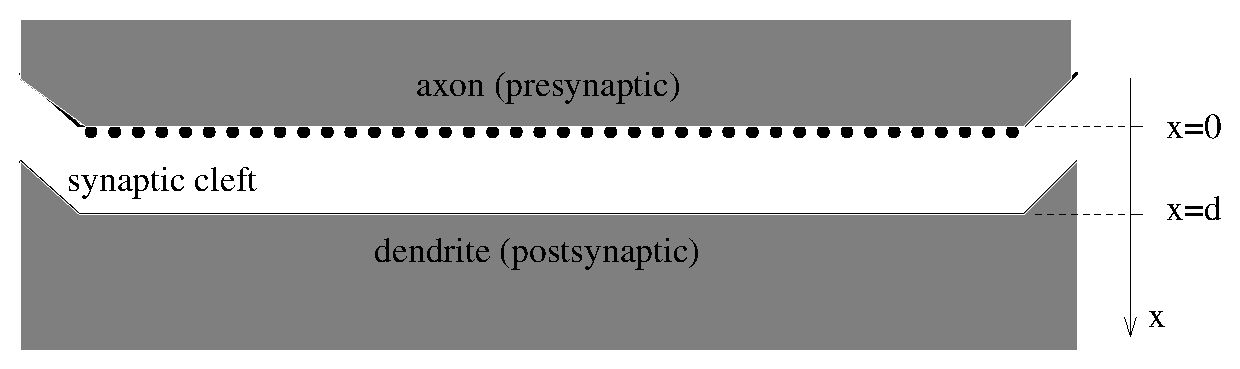
\includegraphics[width=10cm]{FigDiffusion/synaptic_cleft.eps}}
\caption{\small Schematic drawing of the synaptic cleft in our model. The
black dots represent neurotransmitter molecules, and the situation
shown corresponds to the situation immediately after neurotransmitter
release into the synaptic cleft.}
\label{fig:figure3}
\end{figure}
%
%%%%%%%%%%%%%%%%%%%%%%%%%%%%%%%%%%%%%%%%%%%%%%%%%%%%%%%%%%%%%
%
In this case $u({\bf r})=u(x)$, the diffusion equation
reduces to
%
\begin{equation}
\frac{\partial u}{\partial t} = D \frac{\partial^2 u}{\partial x^2}.
\label{eq:diffusion_eq_1D}
\end{equation}\newline
Immediately after the release of a neurotransmitter into the
synaptic cleft ($t=0$) the concentration profile in the $x$-direction
is given by
%
\begin{equation}
u(x,t=0) = N \delta(x),
\label{eq:initial_condition}
\end{equation}
%
where $N$ is the number of particle released into the synaptic cleft
per area of membrane.

To get an idea over the time-dependence of the neurotransmitter
concentration at the postsynaptic side ($x=d$), we can look at the
solution of a ``free'' random walk (i.e., no obstacles or particle
absorbers in either direction). The
solution of Eq.~(\ref{eq:diffusion_eq_1D}) with the initial condition
in Eq.~(\ref{eq:initial_condition}) is given by 
(see Nelson: \emph{Biological Physics}, p. 143 or Lectures notes chapter 12.3)
%
\begin{equation}
u(x,t) = \frac{N}{\sqrt{4 \pi D t}} e^{-x^2/4Dt}\;\;.
\label{eq:solution_delta_1D}
\end{equation}\newline
The concentration at the postsynaptic side $u(d,t)$
approaches 0 in the limit $t \rightarrow 0\;$ and
$t \rightarrow \infty$. 

The above assumption regarding the
neurotransmitter molecules undergoing a ``free'' random walk, is
obviously a simplification. In the true diffusion process in the
synaptic cleft the neurotransmitter molecules will, for example,
occasionally bump into the presynaptic membrane they came from. Also
at the postsynaptic side the neurotransmitters are absorbed by
receptors located on the postsynaptic cell membrane and are thus
(temporally) removed from the solution.

To approach this situation in our mathematical model we can impose the
following boundary and initial conditions with $x\in[0,d]$
%
\begin{equation}
u(x=0,t>0) = u_0, \;\;u(x=d,\mbox{all $t$})=0,
\;\;u(0 < x < d,t < 0) = 0 \;\;.
\label{eq:initial_conditions_2}
\end{equation}
Hereafter we set $d=1$.
This corresponds to that (i) for $t<0$ there are no neurotransmitters
in the synaptic cleft, (ii) for $t>0$ the concentration of
neurotransmitters at the presynaptic boundary of the synaptic
cleft ($x=0$) is kept
\emph{fixed}� at $u=u_0=1$ in our case, and (iii) that the postsynaptic receptors
immediately absorb nearby neurotransmitters so that $u=0$ on the
postsynaptic side of the cleft ($x=d=1$).


The full solution of the diffusion equation with
boundary/initial conditions in Eq.~(\ref{eq:initial_conditions_2})
can be found in a closed form. We will use this solution to test our numerical calculations.


We are thus looking at a one-dimensional
problem 
\[
 \frac{\partial^2 u(x,t)}{\partial x^2} =\frac{\partial u(x,t)}{\partial t}, t> 0, x\in [0,d]
\]
or 
\[
u_{xx} = u_t,
\]
with initial conditions, i.e., the conditions at $t=0$, 
\[
u(x,0)= 0 \hspace{0.5cm} 0 < x < d
\]
with $d=1$ the length of the $x$-region of interest. The 
boundary conditions are 
\[
u(0,t)= 1 \hspace{0.5cm} t > 0,
\]
and 
\[
u(d,t)= 0 \hspace{0.5cm} t > 0.
\]

In this project we want to study the numerical stability of three methods for partial differential equations
(PDEs). 
These methods are 
\begin{enumerate}
\item The explicit forward Euler algorithm with discretized versions of time given by a forward formula and
a centered difference in space resulting in
 \[
u_t\approx \frac{u(x,t+\Delta t)-u(x,t)}{\Delta t}=\frac{u(x_i,t_j+\Delta t)-u(x_i,t_j)}{\Delta t}
\]
and
\[
u_{xx}\approx \frac{u(x+\Delta x,t)-2u(x,t)+u(x-\Delta x,t)}{\Delta x^2},
\]
or
\[
u_{xx}\approx \frac{u(x_i+\Delta x,t_j)-2u(x_i,t_j)+u(x_i-\Delta x,t_j)}{\Delta x^2}.
\]
\item The implicit Backward Euler with
 \[
u_t\approx \frac{u(x,t)-u(x,t-\Delta t)}{\Delta t}=\frac{u(x_i,t_j)-u(x_i,t_j-\Delta t)}{\Delta t}
\]
and
\[
u_{xx}\approx \frac{u(x+\Delta x,t)-2u(x,t)+u(x-\Delta x,t)}{\Delta x^2},
\]
or
\[
u_{xx}\approx \frac{u(x_i+\Delta x,t_j)-2u(x_i,t_j)+u(x_i-\Delta x,t_j)}{\Delta x^2},
\]
\item Finally we use the implicit Crank-Nicolson scheme with 
a time-centered scheme at $(x,t+\Delta t/2)$
 \[
u_t\approx \frac{u(x,t+\Delta t)-u(x,t)}{\Delta t}=\frac{u(x_i,t_j+\Delta t)-u(x_i,t_j)}{\Delta t}.
\]
The corresponding spatial second-order derivative reads
\[
u_{xx}\approx \frac{1}{2}\left(\frac{u(x_i+\Delta x,t_j)-2u(x_i,t_j)+u(x_i-\Delta x,t_j)}{\Delta x^2}+\right.
\]
\[
\left. \frac{u(x_i+\Delta x,t_j+\Delta t)-2u(x_i,t_j+\Delta t)+u(x_i-\Delta x,t_j+\Delta t)}{\Delta x^2}
\right).
\] 
Note well that we are using a time-centered scheme wih $t+\Delta t/2$ as center.
\end{enumerate}
 \begin{enumerate}
\item[a)] Find the closed form solution to this problem. You will need this in order to study the numerical accuracy of your results.  To find the closed-form solution, we will need the  
stationary solution (steady-state solution). The solution to the steady-state problem is on the form $u(x)=Ax+b$. The solution for the steady-state case $u_s$ that obeys the above boundary conditions is 
\[
u_s(x) = 1-x. 
\]
You can use this solution to  define a new function $v(x)=u(x)-u_s(x)$ with boundary conditions
$v(0)=v(d)=0$. The latter is easier to solve both numerically and on a closed form. 
\item[b)] Write down the algorithms for these three methods and the equations you need to implement.
For the implicit schemes show that the equations lead to a tridiagonal matrix system for the new values.
\item [c)] Find the truncation errors of these three schemes and investigate their stability properties.
\item [d)] Implement the three algorithms in the same code and perform tests of the solution 
for these three approaches
for $\Delta x=1/10$, $\Delta x=1/100$ using  $\Delta t$ as dictated by the stability limit of the explicit scheme.
Study the solutions at two time points $t_1$ and $t_2$ where $u(x,t_1)$ is smooth but still significantly curved
and $u(x,t_2)$ is almost linear, close to the stationary state.
Remember that for solving the tridiagonal equations you can use your code from project 1.  
\item[e)] Compare the solutions at $t_1$ and $t_2$ with the closed form result for the continuous problem.
Which of the schemes would you classify as the best?

\item[f)] 
The above problem can be solved using Monte Carlo methods and random walks. We follow here
Farnell and Gibson in Journal of Computational Physics, volume {\bf 208}, pages 253-265 (2005).
Choose a constant step length $l_0=\sqrt{2D\Delta t}$ and equal probability for jumping left and right.
Set up the algorithm for solving the above diffusion problem and write a code to do it.
Compare your results with those from the partial differential equation solution and comment the results.
\item[g)]
Change the above stepsize by using a Gaussian distribution with mean value $1$ and standard deviation $0$. The step length of the random walker is now $l_0=\sqrt{2D\Delta t}\xi$, where $\xi$ is random number chosen from the above Gaussian distribution.  Implement this stepsize to the program from 
f) and compare the results and comment.  
\end{enumerate}

We include for the sake of completeness a code which computes random numbers according to a normal distribution. You can alternatively use the {\bf random} class of C++.

\begin{verbatim}

// function for gaussian random numbers
double gaussian_deviate(long *);

// ran2 for uniform deviates, initialize with negative seed.
double ran2(long *);


// random numbers with gaussian distribution
double gaussian_deviate(long * idum)
{
  static int iset = 0;
  static double gset;
  double fac, rsq, v1, v2;

  if ( idum < 0) iset =0;
  if (iset == 0) {
    do {
      v1 = 2.*ran2(idum) -1.0;
      v2 = 2.*ran2(idum) -1.0;
      rsq = v1*v1+v2*v2;
    } while (rsq >= 1.0 || rsq == 0.);
    fac = sqrt(-2.*log(rsq)/rsq);
    gset = v1*fac;
    iset = 1;
    return v2*fac;
  } else {
    iset =0;
    return gset;
  }
} // end function for gaussian deviates

/*
** The function 
**         ran2()
** is a long periode (> 2 x 10^18) random number generator of 
** L'Ecuyer and Bays-Durham shuffle and added safeguards.
** Call with idum a negative integer to initialize; thereafter,
** do not alter idum between sucessive deviates in a
** sequence. RNMX should approximate the largest floating point value
** that is less than 1.
** The function returns a uniform deviate between 0.0 and 1.0
** (exclusive of end-point values).
*/

#define IM1 2147483563
#define IM2 2147483399
#define AM (1.0/IM1)
#define IMM1 (IM1-1)
#define IA1 40014
#define IA2 40692
#define IQ1 53668
#define IQ2 52774
#define IR1 12211
#define IR2 3791
#define NTAB 32
#define NDIV (1+IMM1/NTAB)
#define EPS 1.2e-7
#define RNMX (1.0-EPS)

double ran2(long *idum)
{
  int            j;
  long           k;
  static long    idum2 = 123456789;
  static long    iy=0;
  static long    iv[NTAB];
  double         temp;

  if(*idum <= 0) {
    if(-(*idum) < 1) *idum = 1;
    else             *idum = -(*idum);
    idum2 = (*idum);
    for(j = NTAB + 7; j >= 0; j--) {
      k     = (*idum)/IQ1;
      *idum = IA1*(*idum - k*IQ1) - k*IR1;
      if(*idum < 0) *idum +=  IM1;
      if(j < NTAB)  iv[j]  = *idum;
    }
    iy=iv[0];
  }
  k     = (*idum)/IQ1;
  *idum = IA1*(*idum - k*IQ1) - k*IR1;
  if(*idum < 0) *idum += IM1;
  k     = idum2/IQ2;
  idum2 = IA2*(idum2 - k*IQ2) - k*IR2;
  if(idum2 < 0) idum2 += IM2;
  j     = iy/NDIV;
  iy    = iv[j] - idum2;
  iv[j] = *idum;
  if(iy < 1) iy += IMM1;
  if((temp = AM*iy) > RNMX) return RNMX;
  else return temp;
}
#undef IM1
#undef IM2
#undef AM
#undef IMM1
#undef IA1
#undef IA2
#undef IQ1
#undef IQ2
#undef IR1
#undef IR2
#undef NTAB
#undef NDIV
#undef EPS
#undef RNMX

// End: function ran2()

\end{verbatim}

\end{document}





















